\documentclass{standalone}

\usepackage{tikz}
\usepackage{tkz-euclide}

\usepackage{times}

\usetikzlibrary {positioning}
\usetikzlibrary{arrows.meta}

\definecolor{accent}{rgb}{0.9,0.9,0.9}

\begin{document}
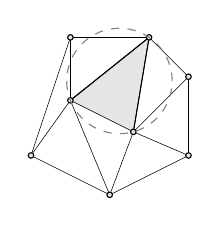
\begin{tikzpicture}[%
  circle/.style={thin, dashed},
]

  \tkzDefPoint(-0.5,0.0){min}
  \tkzDefPoint(2.5,3.0){max}

  \tkzDefPoint(0.0,1.0){v0}
  \tkzDefPoint(1.0,0.5){v1}
  \tkzDefPoint(0.5,1.7){v2}
  \tkzDefPoint(1.5,2.5){v3}
  \tkzDefPoint(0.5,2.5){v4}
  \tkzDefPoint(1.3,1.3){v5}
  \tkzDefPoint(2.0,1.0){v6}
  \tkzDefPoint(2.0,2.0){v7}

  \draw[draw,fill=accent] (v2)--(v3)--(v5);

  % Convex Hull
  \tkzDrawSegments(v0,v1 v1,v6 v6,v7 v7,v3 v3,v4 v4,v0)
  \tkzDrawSegments(v2,v0 v2,v4 v2,v3 v2,v1)
  \tkzDrawSegments(v5,v2 v5,v6 v5,v7 v5,v1 v5,v3)

  \tkzDrawPoints(v0,v1,v2,v3,v4,v5,v6,v7)
  % \tkzLabelPoints(v0,v1,v2,v3,v4,v5,v6,v7)

  \tkzCircumCenter(v2,v3,v5)\tkzGetPoint{M}
  \tkzDrawCircle[circle](M,v2)

\end{tikzpicture}
\end{document}
